\documentclass[aspectratio=169]{beamer}

\usepackage{tikz}
\usepackage{caption}
\setbeamertemplate{caption}[numbered] % Включаем нумерацию для подписей
\newbool{russian}
\booltrue{russian}  % Загружает русскоязычный логотип
\usepackage{theme/theme} % Подгружаем тему

%%% Работа с русским языком и шрифтами
\usepackage[english,russian]{babel}   % загружает пакет многоязыковой вёрстки
\usepackage[no-math]{fontspec}      % подготавливает загрузку шрифтов Open Type, True Type и др.
	\setsansfont{Liberation Sans} 
	\setmonofont{Courier New}
\usepackage{mathspec}
	\setmathsfont(Digits,Latin,Greek)[Numbers={Lining,Proportional}]{Liberation Sans}
	\setmathrm[Numbers={Lining,Proportional}]{Liberation Sans}
\uselanguage{russian}
\languagepath{russian}
\graphicspath{{images/}}  	% Папка с картинками

%%% Информация об авторе и выступлении
\title[Заголовок]{Издательская система \LaTeX{}} 
\subtitle{Статьи, ссылки, системы контроля версий}
\author[Имя автора]{Александр Сергеевич Филипченко \\ \smallskip \scriptsize 797439@edu.rut-miit.ru\\}
\institute{кафедра <<Вычислительные системы, сети и информационная безопасность>>}
\date{\today}

\begin{document}	% Начало презентации

\frame[plain]{\titlepage}	% Титульный слайд

\begin{frame}
\frametitle{План лекции}
	\begin{enumerate} 
	\item Особенности подготовки научных статей в \LaTeX{}
	\item Ссылки на элементы документа
	\item Использование системы контроля версий
 	\item Домашнее задание
\end{enumerate} 
\end{frame}

\section{Особенности подготовки научных статей в \LaTeX{}}

\begin{frame}
\frametitle{Библигорафия. Программный пакет BibLaTeX}
BibLaTeX --- менеджер библиографии.
Состоит из утилиты для работы с \texttt{.bib} файлами \textbf{biber} и пакета \textbf{biblatex}.
Алгоритм работы менеджера библиографии:
\begin{enumerate} 
\item программа \textbf{xelatex} обнаруживает ссылки (команды \texttt{\textbf{\textbackslash cite}}) и подключенные источники в формате в документе и по результатам формирует запрос;
\item программа \textbf{biber} формирует в ответ на запрос LaTeX-файл с нужными библиографическими данными;
\item программа \textbf{xelatex} выполняет проход для расстановки ссылок и добавления списка литературы в документ;
\item программа \textbf{xelatex} выполняет дополнительный проход для перерасстановки номеров страниц и внутренних ссылок в документе.
\end{enumerate} 
\end{frame}

\begin{frame}
\frametitle{Пример использования BibLaTeX}
\medskip
\begin{columns}
\column{0.5\textwidth}
\begin{figure}
  \centering
  \begin{tikzpicture}
    \node[draw=black, line width=1pt, inner sep=0pt] {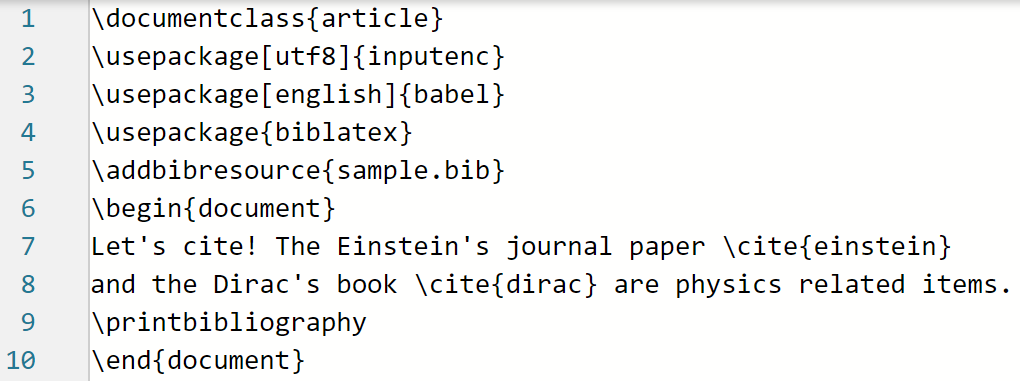
\includegraphics[width=\columnwidth]{BibLatexCode}};
  \end{tikzpicture}
  \caption{Пример исходного кода с использованием BibLaTeX}
\end{figure}
\column{0.5\textwidth}
\begin{figure}
  \centering
  \begin{tikzpicture}
    \node[draw=black, line width=1pt, inner sep=0pt] {
\includegraphics[width=\columnwidth]{BibLatexRes}};
  \end{tikzpicture}
  \caption{Результат сборки}
\end{columns}
\end{frame}

\begin{frame}
\frametitle{Блоки}
	\begin{theorem}[Пифагора]
		Пифагоровы штаны во все стороны равны!!!
		Если $a$ и $b$ "--- длины катетов прямоугольного треугольника, а~$c$ "--- длина гипотенузы, то $a^2+b^2=c^2$.
	\end{theorem}

	\begin{alertblock}{Блок с красным заголовком}
		Содержимое.
	\end{alertblock}

	\begin{exampleblock}{Блок с зеленым заголовком}
		Содержимое.
	\end{exampleblock}
\end{frame}


\end{document}
